\documentclass[11pt]{article}

\usepackage[margin=1in]{geometry}
\usepackage{setspace}
\onehalfspacing
\usepackage{graphicx}
\usepackage{listings}
\usepackage{float}

% DOCUMENT INFORMATION =================================================
\title {ECEN 429: Introduction to Digital Systems Design Laboratory \\ North Carolina Agricultural and Technical State University \\ Department of Electrical and Computer Engineering} % Declare Title
\author{Chris Cannon} % Declare authors
\date{February 8, 2018}
% ======================================================================

\begin{document}
	
\maketitle

\begin{center}
	Lab 3 Prelab
\end{center}

\pagebreak

\section{Introduction}

The objective of this lab is to use the Vivado Design Suite to perform more complex tasks on the Basys3 Development board. For the first time, we will introduce buffers, exclusive-OR gates, and multiplexers. These digital elements represent higher-level digital design, and allow us to create more complex digital circuits than we have in the past.

\section{Background, Design Solution, and Results}

\subsection{Problem 1 2-bit Comparator}

\begin{lstlisting}[language=VHDL]
entity comparator is port(a1, a0, b1, b0 : in bit; q : out bit);
end entity comparator;

architecture comp_arch of comparator is
signal tmp1 : bit;
signal tmp2 : bit;
signal tmp3 : bit;
signal tmp4 : bit;
begin
		tmp1 <= a1 xor b1;
		tmp2 <= a0 xor b0;
		tmp3 <= not tmp1;
		tmp4 <= not tmp2;
		q <= tmp3 and tmp4;
end architecture comp_arch;
\end{lstlisting}


\subsection{Problem 2 Tri-State Buffer}

\subsubsection{One-bit Tri-state Buffer}

\begin{table}[h]
\begin{center}
	\begin{tabular}{| l | l | l |}
		\hline
		x & c & z \\ \hline
		0 & 0 & 0 \\ \hline
		0 & 1 & 0 \\ \hline
		1 & 0 & 0 \\ \hline
		1 & 1 & 1 \\ \hline
	\end{tabular}
	\caption{\label{tab:triStateTruthTable}Truth Table for Tri-State Buffer assuming active HIGH.}
\end{center}	
\end{table}

\begin{lstlisting}[language=VHDL]
	z <= x and c;
\end{lstlisting}


\subsubsection{Two-bit Tri-state Buffer}

\begin{figure}[H]
\begin{center}
	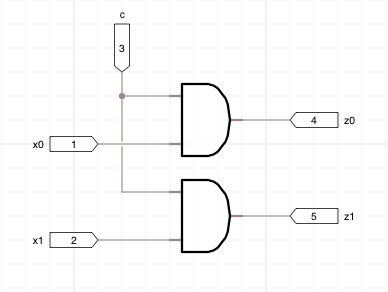
\includegraphics{img3_1.png}
	\caption{\label{fig:triStateSchematic} Schematic for 2-bit Tri-State buffer assuming active HIGH.}
\end{center}
\end{figure}

\begin{lstlisting}[language=VHDL]
entity two_bit_tri is port(x0, x1, c : in bit; z0, z1 : out bit);
end entity two_bit_tri;
	
architecture tri_arch of two_bit_tri is
begin
	z0 <= x0 and c;
	z1 <= z1 and c;
end architecture tri_arch;
\end{lstlisting}

\subsection{Problem 3 2:1 Multiplexer}

\begin{lstlisting}[language=VHDL]
entity mux is port(sum, cout, control : in bit; x : out bit);
end entity mux;

architecture mux_arch of mux is
begin
	output <= sum when (control = '0') else cout;	
\end{lstlisting}

\section{Conclusion}

After completing these exercises, this lab does appear to operate at a higher level of complexity than the previous labs. After completing this lab, I will have experienced implementing devices that can be used in very practical designs. What struck me most in these exercises was that even though the devices being implemented are interesting and perform relatively complex conceptual tasks, the implementation for them is quite simple.

\end{document}